\section{Fonctions d'interpolation classiques}

La précision et l'efficacité de la méthode des éléments finis repose grandement sur le choix judicieux des fonctions de
forme $\phi$.

Communément, le choix, pour des problèmes en traction/compression, se fait entre des fonctions linéaires et
quadratiques.

Il est nécessaire, lors de la comparaison de ces deux alternatives, de prendre en compte non pas le nombre d'éléments
mais bien le nombre de degrés de liberté\footnote{Points où sont calculées les valeurs des champs utilisées ensuite pour
l'interpolation.}. En effet, le concept derrière l'interpolation avec des polynômes est toujours le même : pour un
polynôme de degré $N$, il faut $N+1$ point.

\subsection{Éléments Linéaires}

La première interpolation possible utilise des fonctions affines. L'idée est alors d'écrire :

$$p = p_1\phi_1(x) + p_2\phi_2(x)$$

Avec $p_{1,2}$ les valeurs du champ à chaque extrémité $x_{1,2}$ et $\phi_{1,2}$ nulles en $x_{2,1}$ et égales à l'unité
en $x_{1,2}$. Ainsi, les deux fonctions ont le profil présenté en figure~\ref{fig:FEM:lin_shape_fun}.

\begin{figure}[!ht]
	\centering
	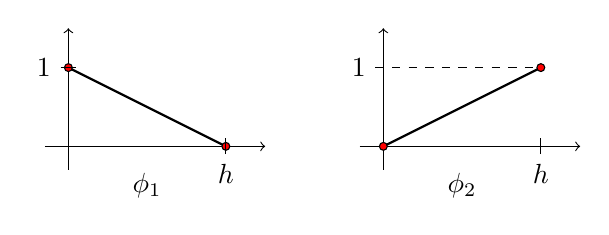
\begin{tikzpicture}
	\def\h{2};

	% PHI 1
	\draw[thick] plot [domain=0:\h] (\x,{1-\x/\h});
	\draw[->] (-.3,0) -- (\h+.5,0);
	\draw[->] (0,-.3) -- (0,1.5);
	\draw[fill=red] (0,1) circle (.05);
	\draw[fill=red] (\h,0) circle (.05);
	\draw (-.1,1) node[left] {$1$} --++(.2,0);
	\draw (\h,-.1) node[below] {$h$} --++(0,.2);
	\draw (\h*.5,-.5) node {$\phi_1$};

	% PHI 2
	\begin{scope}[shift={(\h+2,0)}]
		\draw[thick] plot [domain=0:\h] (\x,{\x/\h});
		\draw[->] (-.3,0) -- (\h+.5,0);
		\draw[->] (0,-.3) -- (0,1.5);
		\draw[fill=red] (0,0) circle (.05);
		\draw[fill=red] (\h,1) circle (.05);
		\draw[dashed] (-.1,1) node[left] {$1$} -- (\h,1);
		\draw (\h,-.1) node[below] {$h$} --++(0,.2);
		\draw (\h*.5,-.5) node {$\phi_2$};
	\end{scope}
\end{tikzpicture}


	\caption{\label{fig:FEM:lin_shape_fun}Présentation des fonctions de forme linéaires utilisées. L'élément est ici considéré
	de longueur $h$.}
\end{figure}

Pour un élément de longueur $h$, les expressions des fonctions de forme linéaires sont donc :

\begin{equation*}
	\phi_1(x) = 1-\frac{x}{h} \quad;\quad \phi_2(x) = \frac{x}{h}
\end{equation*}


\subsection{Éléments quadratiques}

Une deuxième possibilité est d'utiliser une interpolation quadratique (polynôme de degré 2). Pour ce faire, en plus des
deux points précédement considérés, il faudra en utiliser un troisième situé au centre de l'élément. Les fonctions de
formes sont alors au nombre de trois et le champ est approximé par :

$$p(x) = p_1\phi_1(x) + p_2\phi_2(x) + p_3\phi_3(x)$$

Les expressions des fonctions d'ordre 2 sont données ci-après : elles sont calculées en utilisant le polynôme
interpolateur de Lagrange. Les graphes sont présentés en figure~\ref{fig:FEM:shape_fun_quad}.

\begin{equation*}
	\phi_1(x) = \frac{(h-2x)(h-x)}{h^2} \quad,\quad \phi_2(x) = \frac{-4x(x-h)}{h^2} \quad,\quad \phi_3(x) = \frac{x(2x-h)}{h^2}
\end{equation*}

\begin{figure}[!ht]
	\centering
	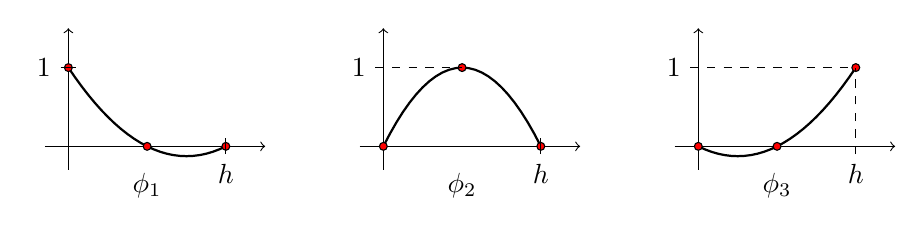
\begin{tikzpicture}
	\def\h{2};

	% PHI 1
	\draw[thick] plot [domain=0:\h] (\x,{((\h-2*\x)*(\h-\x))/(\h*\h)});
	\draw[->] (-.3,0) -- (\h+.5,0);
	\draw[->] (0,-.3) -- (0,1.5);
	\draw[fill=red] (0,1) circle (.05);
	\draw[fill=red] (\h*.5,0) circle (.05);
	\draw[fill=red] (\h,0) circle (.05);
	\draw (-.1,1) node[left] {$1$} --++(.2,0);
	\draw (\h,-.1) node[below] {$h$} --++(0,.2);
	\draw (\h*.5,-.5) node {$\phi_1$};

	% PHI 2
	\begin{scope}[shift={(\h+2,0)}]
		\draw[thick] plot [domain=0:\h] (\x,{(-4*\x*(\x-\h))/(\h*\h)});
		\draw[->] (-.3,0) -- (\h+.5,0);
		\draw[->] (0,-.3) -- (0,1.5);
		\draw[fill=red] (0,0) circle (.05);
		\draw[fill=red] (\h*.5,1) circle (.05);
		\draw[fill=red] (\h,0) circle (.05);
		\draw[dashed] (-.1,1) node[left] {$1$} -- (\h*.5,1);
		\draw (\h,-.1) node[below] {$h$} --++(0,.2);
		\draw (\h*.5,-.5) node {$\phi_2$};
	\end{scope}

	% PHI 2
	\begin{scope}[shift={({2*(\h+2)},0)}]
		\draw[thick] plot [domain=0:\h] (\x,{(\x*(2*\x-\h))/(\h*\h)});
		\draw[->] (-.3,0) -- (\h+.5,0);
		\draw[->] (0,-.3) -- (0,1.5);
		\draw[fill=red] (0,0) circle (.05);
		\draw[fill=red] (\h*.5,0) circle (.05);
		\draw[fill=red] (\h,1) circle (.05);
		\draw[dashed] (-.1,1) node[left] {$1$} -- (\h,1);
		\draw[dashed] (\h,-.1) node[below] {$h$} -- (\h,1);
		\draw (\h*.5,-.5) node {$\phi_3$};
	\end{scope}
\end{tikzpicture}

	\caption{\label{fig:FEM:shape_fun_quad}Présentation des fonctions de forme quadratiques utilisées. L'élément est ici considéré
	de longueur $h$.}
\end{figure}

Avec 3 fonctions d'interpolation, les matrices élémentaires seront de taille 3 (comportant ainsi 9 éléments).

\subsection{Note sur l'implémentation}

La méthode des éléments finis fait appel aux intégrales des produits de fonction de forme.

Dans le cas où tous les éléments sont les mêmes, il est possible de calculer une seule fois les matrices élémentaires (à
la main par exemple) et de réaliser l'assemblage à partir de ces patrons.

Il faut noter que les matrices élémentaires sont symétriques et que les symétries inhérentes aux fonctions de forme
permettent de réduire grandement le nombre de calculs à effectuer : de 9 éléments dans la matrice élémentaire pour des
éléments quadratiques, seuls 5 devront être calculés pour la remplir complètement. 

Si toutefois l'objectif est d'étudier la convergence de la méthode, alors il faudra recalculer les fonctions pour les
$N$ itérations ou paramètrer les fonctions de forme avec un paramètre $h$.

Toujours est il qu'il est aussi possible de s'épargner des calculs peu épanouissants en utilisant des techniques
d'intégration numérique pour obtenir les valeurs des intégrales : dans la suite et les scripts utilisés pour obtenir les
résultats ici, l'intégration est faite soit à la main --- rare, ou plus généralement en utilisant la quadrature de
Gauss.

